
\documentclass{article}
\usepackage{graphicx}
\usepackage{listings}
\usepackage{xcolor}
\usepackage{hyperref}
\usepackage[a4paper, margin=0.75in]{geometry}

\lstdefinestyle{customC}{
    language=C++,
    basicstyle=\ttfamily\small,
    keywordstyle=\color{blue}\bfseries,
    commentstyle=\color{gray}\itshape,
    stringstyle=\color{red},
    numbers=left,
    numberstyle=\tiny\color{gray},
    stepnumber=1,
    frame=single,
    tabsize=4,
    breaklines=true,
    showstringspaces=false,
    captionpos=b,
}

\lstset{style=customC}

\title{Lab: Matrix Sum}
\author{111062117, Hsiang-Sheng Huang}

\begin{document}

\maketitle

\section{Why is the Original Program Slow?}
The original program suffers from poor CPU cache utilization due to cache locality issues arising from an inefficient access pattern. Although the matrix, defined as \texttt{mat[N][M]}, is stored in row-major order, the summation loop accesses elements in a column-first manner (using \texttt{mat[j][i]}). This causes each jump in the j index to access different cache lines, resulting in frequent cache misses and high cache miss rates, which substantially slow down the computation.

\section{Verification with \texttt{perf}}
\begin{figure}[h]
    \centering
    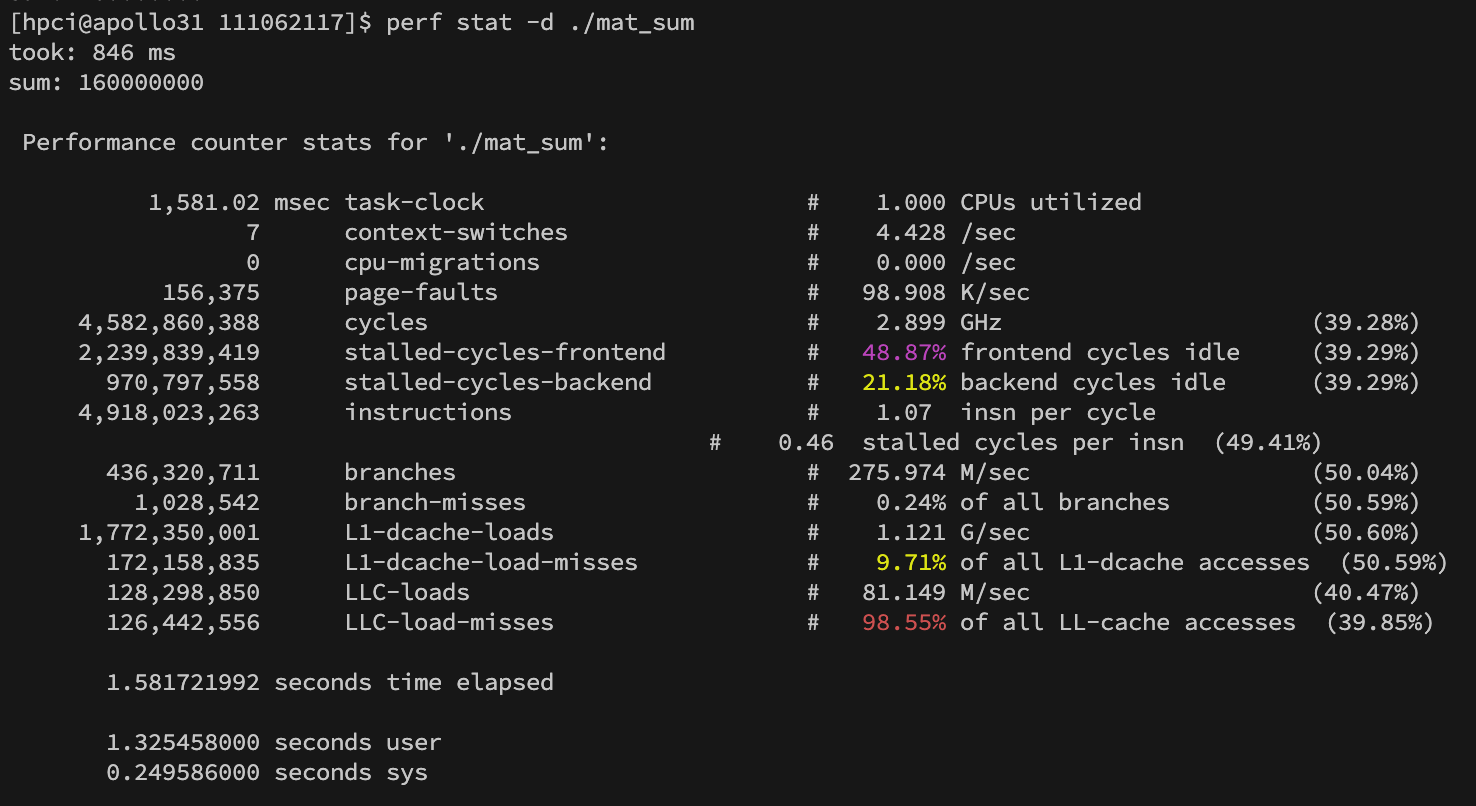
\includegraphics[width=0.7\linewidth]{./img/img-1.png}
    \caption{Performance before optimization}
\end{figure}

We measure the program's efficiency using \texttt{perf}:

\begin{itemize}
    \item \textbf{L1 data cache misses}: Indicates how often requested data is not found in L1 cache.
    \item \textbf{LLC (Last Level Cache) misses}: Shows how frequently memory accesses result in expensive main memory fetches.
    \item \textbf{Branch mispredictions and CPU cycles}: To measure overall efficiency.
\end{itemize}

The high cache miss rates and CPU cycles suggest poor cache utilization and memory access patterns, leading to slow performance.

The further analysis will be shown in the Section~\ref{sec:verify}.

\section{Optimizing Performance}
To improve performance, we modify the program to utilize \textbf{row-major access}:

\begin{lstlisting}
for (int i = 0; i < N; i++) {
    for (int j = 0; j < M; j++) {
        sum += mat[i][j]; // Access matrix elements in row-major order
    }
}
\end{lstlisting}

By accessing matrix elements in row-major order, we ensure that consecutive elements are stored in contiguous memory locations. This enhances \textbf{cache locality} and reduces cache misses, leading to improved performance.

\section{Verify Performance Improvements}
\label{sec:verify}

We compare execution times and cache performance using \texttt{perf} before and after optimizations:

\begin{figure}[h]
    \centering
    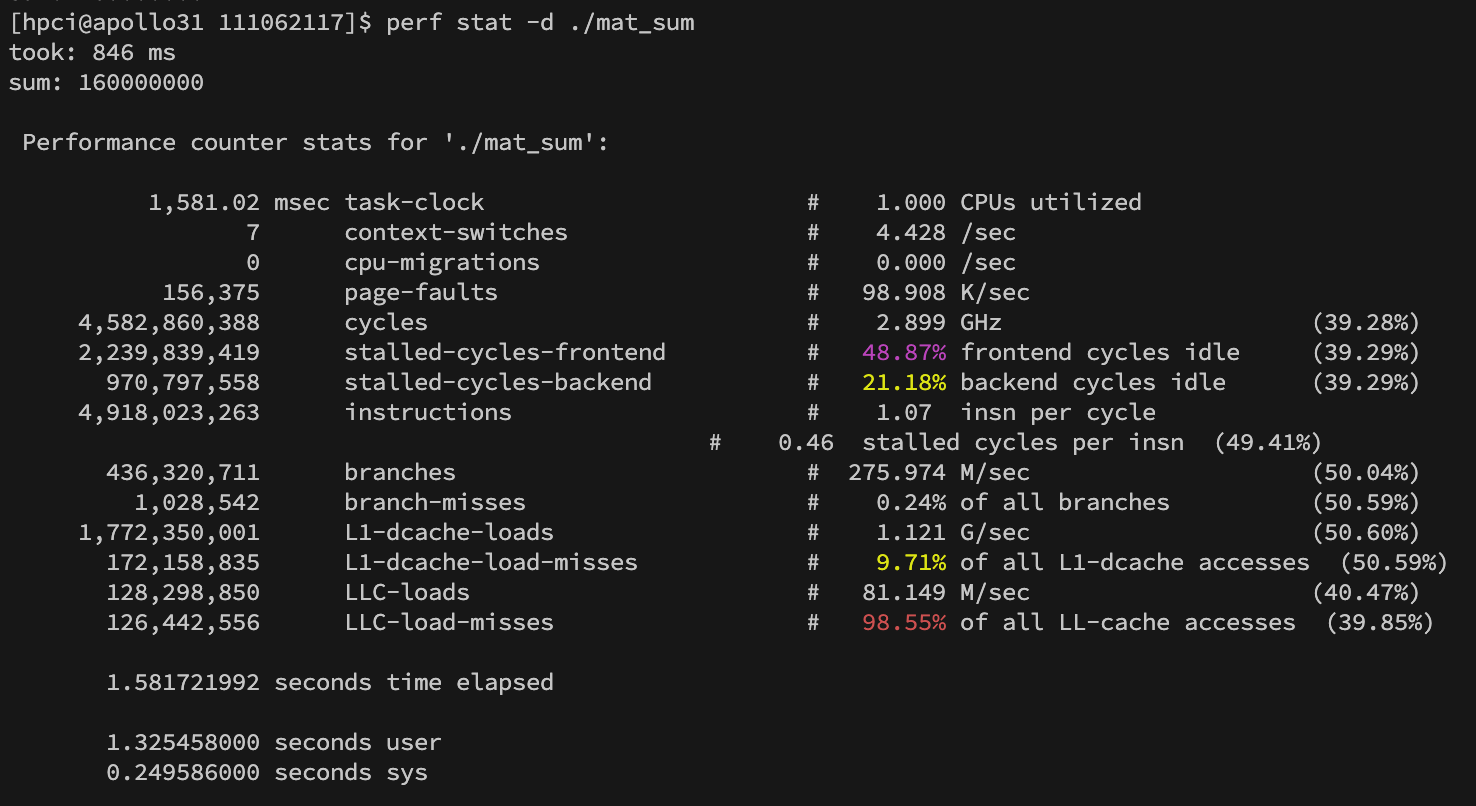
\includegraphics[width=0.7\linewidth]{./img/img-1.png}
    \caption{Performance before optimization}
\end{figure}

\begin{figure}[h]
    \centering
    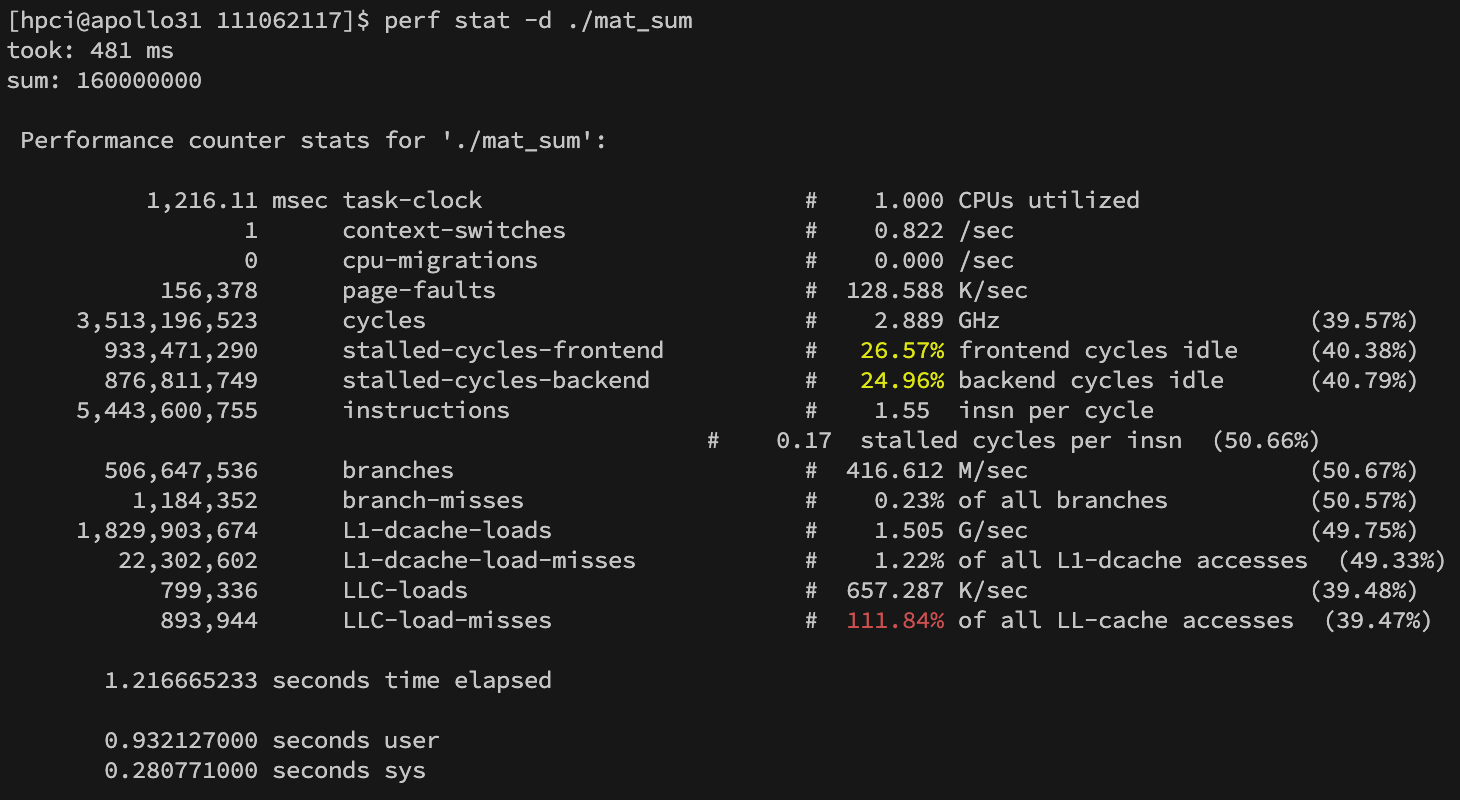
\includegraphics[width=0.7\linewidth]{./img/img-2.png}
    \caption{Performance after optimization}
\end{figure}

To evaluate the impact of cache optimization, we compare the performance metrics using \texttt{perf stat -d ./mat\_sum}. Below are the key observations:

\subsection{Total Execution Time}
Before optimization, the program took \textbf{1.5817 seconds}, whereas after optimization, it was reduced to \textbf{1.2167 seconds}, yielding an improvement of approximately \textbf{23.1\%}.

\subsection{L1 Data Cache (L1-dcache)}
\begin{itemize}
    \item \textbf{Before Optimization:}
    \begin{itemize}
        \item \texttt{L1-dcache-loads}: 1,772,350,001
        \item \texttt{L1-dcache-load-misses}: 172,158,835 (\textbf{9.71\% miss rate})
    \end{itemize}
    \item \textbf{After Optimization:}
    \begin{itemize}
        \item \texttt{L1-dcache-loads}: 1,829,903,674
        \item \texttt{L1-dcache-load-misses}: 22,302,602 (\textbf{1.22\% miss rate})
    \end{itemize}
    \item \textbf{Improvement:} L1 cache miss rate dropped significantly from \textbf{9.71\% to 1.22\%}, indicating better memory locality and efficient cache utilization.
\end{itemize}

\subsection{Last Level Cache (LLC)}
\begin{itemize}
    \item \textbf{Before Optimization:}
    \begin{itemize}
        \item \texttt{LLC-loads}: 128,298,850
        \item \texttt{LLC-load-misses}: 126,442,556 (\textbf{98.55\% miss rate})
    \end{itemize}
    \item \textbf{After Optimization:}
    \begin{itemize}
        \item \texttt{LLC-loads}: 799,336
        \item \texttt{LLC-load-misses}: 893,944 (\textbf{111.84\% miss rate})
    \end{itemize}
    \item \textbf{Observation:} LLC accesses have decreased significantly, reducing expensive memory accesses. The increase in LLC miss rate is due to fewer total accesses.
\end{itemize}

\subsection{CPU Stalls and Efficiency}
\begin{itemize}
    \item \textbf{Before Optimization:}
    \begin{itemize}
        \item \texttt{stalled-cycles-frontend}: 48.87\%
        \item \texttt{stalled-cycles-backend}: 21.18\%
    \end{itemize}
    \item \textbf{After Optimization:}
    \begin{itemize}
        \item \texttt{stalled-cycles-frontend}: 26.57\%
        \item \texttt{stalled-cycles-backend}: 24.96\%
    \end{itemize}
    \item \textbf{Improvement:} The reduction in \texttt{frontend stalls} indicates that the CPU spends less time waiting for instructions, thus improving execution efficiency.
\end{itemize}

\subsection{Conclusion}
The optimization significantly improved cache utilization, reducing execution time by \textbf{23\%}. The key takeaways are:
\begin{itemize}
    \item \textbf{Lower L1 cache miss rate} from \textbf{9.71\% to 1.22\%}.
    \item \textbf{Fewer LLC accesses}, reducing main memory latency.
    \item \textbf{Better CPU efficiency}, with lower frontend stalls.
\end{itemize}

\end{document}